\lfoot{Autor: Fitim Faiku}
\subsubsection{Kompatible Geräte}
\label{subsec:device-compability}

Android kann auf vielen verschiedenen Plattformen, wie Handys oder Tablets laufen.
Als Entwickler bietet das breite Spektrum von Geräten ein enormes potenzielles Publikum.
Um auf diesen unterschiedlichen Plattformen reibungslos zu funktionieren muss eine App einige Feature Variabilitäten tolerieren und eine 
flexible Benutzeroberfläche zu Verfügung stellen. 

Um das zu ermöglichen bietet Android die Möglichkeit, verschiedene XML Layouts zu erstellen um verschiedene Bildschirmgrößen anzusprechen.

Beim Programmieren der App kann auch die minimale und maximale kompatible Android-Version/SDK-Version des Devices eingestellt werden, wobei hier eine möglichst umfangreiche Auswahl der Versionen einen größeren Umfang an Nutzern erzielen.

\begin{figure}[!htb]\centering
	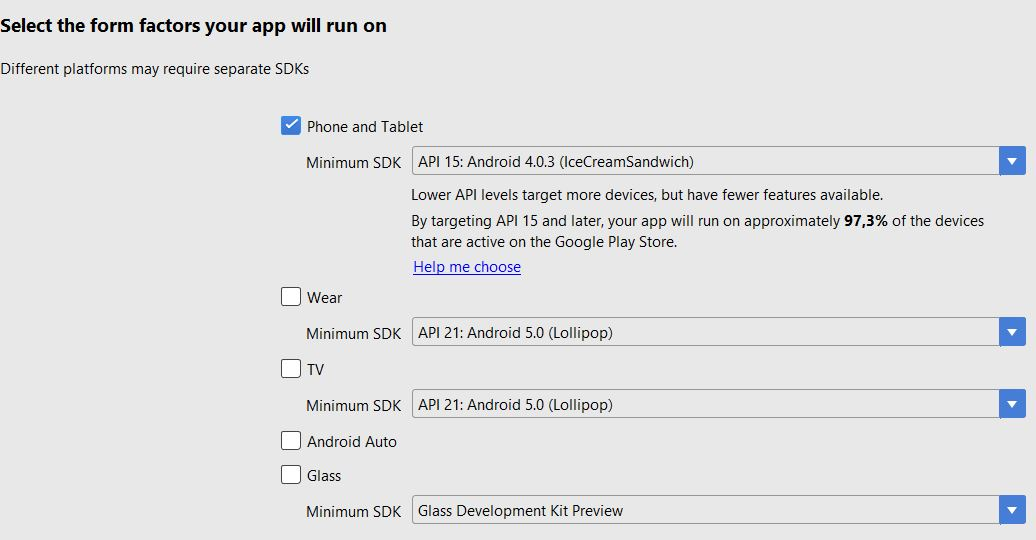
\includegraphics[width=1.0 \textwidth]{images/MinMaxVers}
	\caption{Eintragen der min max API-Version}\label{Fig:min-max Version}
\end{figure}




\clearpage % DO NOT REMOVE